\subsection{Cabibbo Angle}
%-----------------------------------------------------------------------------

\begin{corollary}{Cabibbo Angle}{Cabibbo}
The Cabibbo parameter is fixed by the birefringence invariant $\phiz$:
\begin{equation}
\lambda \equiv \sin\theta_C
:= \sqrt{\phiz(1-\phiz)}
:= \sqrt{4\pi\beta_{\text{rad}}\left(1-4\pi\beta_{\text{rad}}\right)}
:= 0.22437623688472177\ldots
\end{equation}
Compared to the PDG reference value, this is a sub-permille level deviation (status: solid).
\end{corollary}

\begin{tcolorbox}[colback=gray!5, colframe=gray!60, 
    title={\textbf{CKM Conventions and Scale (Clarification)}}, fonttitle=\bfseries\small]
\textbf{Convention:} We use the PDG/Wolfenstein identification $\lambda = |V_{us}|$.

\textbf{Scope:} TFPT uses the Cabibbo relation above as a low-energy prediction anchored in $\phiz$; it does \emph{not} compute the full CKM fit, RG evolution of CKM parameters, or threshold matching.
Any extension to a full CKM prediction must specify scheme and reference scale (e.g.\ $\overline{\mathrm{MS}}$ at $M_Z$) and propagate experimental/hadronic uncertainties.
\textbf{Disposition:} A publication-grade CKM matrix reconstruction is treated as a separate, RG-complete program; the verification suite ships a deterministic RG-dressed texture pipeline (PyR@TE-generated two-loop betas with explicit threshold bookkeeping and a declared reference-scale comparison) to make the conventions and extraction steps explicit.
\end{tcolorbox}

\begin{tcolorbox}[colback=gray!5, colframe=gray!60,
    title={\textbf{Convention Lock (Holdout Protocol; avoids ``convention shopping'')}}, fonttitle=\bfseries\small]
\textbf{Problem:} Even if all candidates are discrete, a ``pick the smallest $\chi^2$'' rule can accidentally select a convention that fits a subset of entries but fails badly on the remaining ones.

\textbf{Suite protocol (unconventional audit):} We therefore run a deterministic holdout scan (\texttt{ux\_flavor\_holdout\_search}) with
\[
\text{fit keys}=\{V_{ud},V_{us},V_{cd},V_{cs},V_{cb},V_{ts},V_{tb}\},\qquad
\text{holdout}=\{V_{ub},V_{td}\}.
\]
\textbf{Outcome:} The best-fit candidate (\texttt{koide\_pi\_over\_12}) achieves $\chi^2_{\rm fit}\simeq 2.48$ but catastrophically fails the holdout ($\chi^2_{\rm holdout}\simeq 186$). The stable convention is \texttt{pi\_times\_1\_minus\_delta} with $\chi^2_{\rm total}\simeq 5.11$ and $\chi^2_{\rm holdout}\simeq 2.38$, and is treated as the preferred default (\texttt{v107sm\_default}) rather than as a post-hoc pick.
\end{tcolorbox}

\begin{figure}[H]
\centering
\begin{tikzpicture}
\begin{groupplot}[
    group style={group size=2 by 1, horizontal sep=1.2cm},
    ybar,
    bar width=10pt,
    width=0.48\textwidth,
    height=0.42\textwidth,
    xmin=0.5, xmax=4.5,
    xtick={1,2,3,4},
    xticklabels={
        \texttt{pi\_times\_1\_minus\_delta},
        \texttt{koide\_pi\_over\_12},
        \texttt{pi\_times\_delta},
        \texttt{2pi\_times\_delta}
    },
    x tick label style={rotate=25, anchor=east, font=\scriptsize},
    grid=both,
    legend style={font=\scriptsize},
]
\nextgroupplot[
    title={fit $\chi^2$},
    ylabel={$\chi^2_{\rm fit}$},
    ymin=0, ymax=6.2,
]
\addplot coordinates {
    (1,2.7273332483922754)
    (2,2.479112421420773)
    (3,4.05899978942247)
    (4,5.162857066748017)
};

\nextgroupplot[
    title={holdout $\chi^2$},
    ylabel={$\chi^2_{\rm holdout}$},
    ymode=log,
    ymin=1, ymax=1000,
]
\addplot coordinates {
    (1,2.378204155291164)
    (2,168.10522472179576)
    (3,173.9429926914698)
    (4,347.6044990986585)
};
\end{groupplot}
\end{tikzpicture}
\caption{Unconventional holdout scan (\texttt{ux\_flavor\_holdout\_search}): discrete CKM convention candidates ranked by fit-$\chi^2$ with explicit holdout penalties.}
\end{figure}

\subsubsection{Suite benchmark: RG-dressed CKM pipeline (explicit conventions)}
The shipped suite includes a deterministic CKM reconstruction pipeline with declared UV textures, two-loop RG dressing, and a reference-scale comparison at $M_Z$ (module \texttt{ckm\_full\_pipeline}). The baseline benchmark gives a CKM matrix close to PDG at the level quantified by the reported $\chi^2=\num{\TFPTCKMchiTwo}$.

\begin{tcolorbox}[colback=yellow!3, colframe=yellow!60!black, breakable,
title={\textbf{Benchmark hygiene: explicit external phase override (no hidden fit)}}, fonttitle=\bfseries\small]
\textbf{What is compared:} the pipeline benchmarks the \emph{magnitudes} $|V_{ij}|$ at a declared reference scale (native $m_t$, comparison at $M_Z$) under a fully explicit RG/matching policy.

\textbf{External anchor (declared):} the CKM CP phase is currently anchored by a declared convention,
\[
\delta_{\mathrm{CKM}} := \delta_{\mathrm{CP}}(\mathrm{PDG}) = \pi/3,
\]
i.e.\ the suite runs in \texttt{delta\_mode=external\_delta\_cp\_override} for this benchmark (see \codepath{tfpt-suite/out/ckm_full_pipeline/report.txt}).

\textbf{Status:} this section is therefore a \emph{benchmark pipeline} (deterministic, audited, no continuous fitting), not a closed TFPT prediction of $\delta_{\mathrm{CKM}}$. Replacing the external phase override by a discrete topological phase selection is an explicit roadmap item.
\end{tcolorbox}

\TFPTCKMMatrixBlock

\TFPTYukawaTextureBlock

\TFPTYukawaHeatmapPlot

\subsubsection{Rare Kaon Decays: $K\to\pi\nu\bar{\nu}$ as a clean flavor null test}
\label{sec:rare-kaon}

The ultra clean modes $K^+ \to \pi^+ \nu\bar{\nu}$ and $K_L \to \pi^0 \nu\bar{\nu}$ provide
a stringent test of the TFPT flavor architecture, because long-distance hadronic uncertainties
are strongly suppressed (see the companion note \cite{rareKaonNote2025}).

We use the standard short-distance expression
\begin{equation}
\mathrm{BR}(K^+ \to \pi^+ \nu\bar{\nu}) =
\kappa_+\left[
\left(\frac{\mathrm{Im}\,\lambda_t}{\lambda^5}X_t\right)^2+
\left(\frac{\mathrm{Re}\,\lambda_c}{\lambda}P_c+\frac{\mathrm{Re}\,\lambda_t}{\lambda^5}X_t\right)^2
\right],
\end{equation}
with $\lambda_i := V_{is}^\ast V_{id}$ and $\lambda \equiv |V_{us}|$. The CKM inputs for
$\lambda_t$ and $\lambda_c$ are taken from the benchmark matrix in Sec.~7.3.1
(suite \texttt{ckm\_full\_pipeline}), and we adopt the Buras normalization in which the
short-distance prefactors $\kappa_+$ and $\kappa_L$ already include the overall $\lambda^8$
scaling and phase-space/isospin factors (so the explicit $\lambda$ and $\lambda^5$ factors
above are not double-counted).

For the neutral mode we use
\begin{equation}
\mathrm{BR}(K_L \to \pi^0 \nu\bar{\nu}) =
\kappa_L\left(\frac{\mathrm{Im}\,\lambda_t}{\lambda^5}X_t\right)^2.
\end{equation}

Using the TFPT Cabibbo value from $\phiz$,\footnote{The companion note
\cite{rareKaonNote2025} uses the v2.5 Cabibbo approximation
$\lambda \simeq \sqrt{\varphi_0}(1-\varphi_0/2)$; the difference is sub-permille and does not
change the quoted bands.}
\begin{equation}
\lambda_{\mathrm{TFPT}}=\sqrt{\phiz(1-\phiz)}=0.2243762369\ldots,
\end{equation}
and benchmark loop inputs $(X_t,P_c,\kappa_+,\kappa_L)$ as in the kaon literature
\cite{brod2021,buras2022,na622024},
the resulting branching ratios are
\begin{equation}
\mathrm{BR}(K^+ \to \pi^+ \nu\bar{\nu})_{\mathrm{TFPT}} = 8.22\times 10^{-11},
\qquad
\mathrm{BR}(K_L \to \pi^0 \nu\bar{\nu})_{\mathrm{TFPT}} = 2.65\times 10^{-11}.
\end{equation}

\begin{figure}[H]
\centering
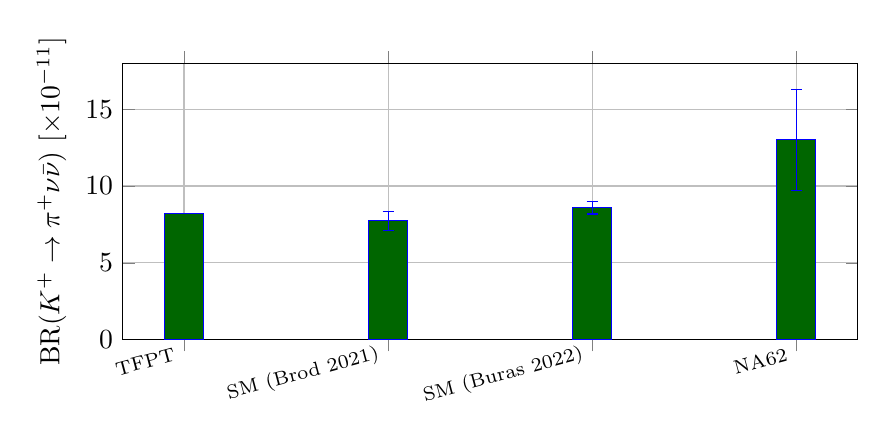
\begin{tikzpicture}
\begin{axis}[
    ybar,
    bar width=14pt,
    width=0.9\linewidth,
    height=0.42\linewidth,
    ymin=0, ymax=18,
    symbolic x coords={TFPT, SM (Brod 2021), SM (Buras 2022), NA62},
    xtick=data,
    x tick label style={rotate=15, anchor=east, font=\scriptsize},
    ylabel={BR($K^+\to\pi^+\nu\bar{\nu}$) [$\times 10^{-11}$]},
    grid=major,
    error bars/y dir=both,
    error bars/y explicit,
]
\addplot+[fill=green!40!black] coordinates {
    (TFPT,8.22) +- (0.0,0.0)
    (SM (Brod 2021),7.73) +- (0.61,0.61)
    (SM (Buras 2022),8.60) +- (0.42,0.42)
    (NA62,13.0) +- (3.3,3.3)
};
\end{axis}
\end{tikzpicture}
\caption{Rare kaon decay comparison: TFPT prediction for $\mathrm{BR}(K^+ \to \pi^+ \nu\bar{\nu})$ versus Standard Model expectations and NA62 \cite{brod2021,buras2022,na622024}.}
\label{fig:kaon_bar}
\end{figure}

\begin{figure}[H]
\centering
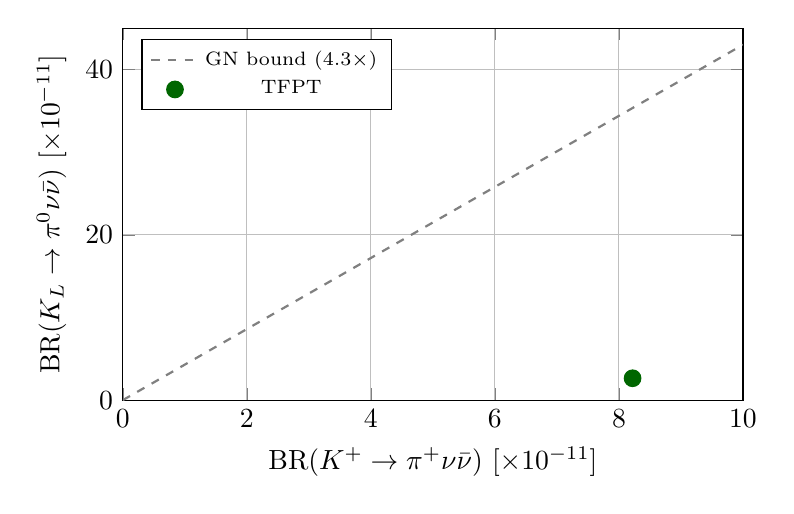
\begin{tikzpicture}
\begin{axis}[
    width=0.78\linewidth,
    height=0.52\linewidth,
    xmin=0, xmax=10,
    ymin=0, ymax=45,
    xlabel={BR($K^+\to\pi^+\nu\bar{\nu}$) [$\times 10^{-11}$]},
    ylabel={BR($K_L\to\pi^0\nu\bar{\nu}$) [$\times 10^{-11}$]},
    grid=major,
    legend style={font=\scriptsize},
    legend pos=north west
]
    \addplot[gray, dashed, thick] coordinates {(0,0) (10,43)};
    \addlegendentry{GN bound ($4.3\times$)}

\addplot[only marks, mark=*, mark size=3pt, green!40!black] coordinates {(8.22,2.65)};
    \addlegendentry{TFPT}
\end{axis}
\end{tikzpicture}
\caption{Charged vs.\ neutral rare-kaon correlation with the Grossman--Nir bound line.}
\label{fig:kaon_correlation}
\end{figure}

%-----------------------------------------------------------------------------
\subsection{PMNS Neutrino Mixing: TM1 Pattern}
%-----------------------------------------------------------------------------

\begin{tcolorbox}[colback=blue!3, colframe=blue!50!black, 
    title={\textbf{PMNS: closed sub-block vs.\ open interface}}, fonttitle=\bfseries]
TFPT provides a \emph{closed} prediction for $(\theta_{13},\theta_{12})$ via a single kernel identity plus the TM1 pattern. The remaining PMNS degrees of freedom $(\theta_{23},\delta_{\mathrm{CP}})$ are treated as an \emph{open interface} requiring explicit Z$_3$-breaking and (eventually) correlated Yukawa/RG treatment; they must not be read as closed predictions at this stage.

\textbf{Key identity} (from $\beta_{\text{rad}} = \phiz/(4\pi)$):
\begin{equation}
    \sin^2\theta_{13} = 4\pi\,\beta_{\text{rad}}\, e^{-\gamma(0)} 
    = \frac{\phiz}{8\pi\cthree}\, e^{-\gamma(0)} = \num[round-mode=places,round-precision=6]{\TFPTsinSqThetaThirteen}
\end{equation}
where $\gamma(0)=g/(g+1)=5/6$ is fixed by holonomy degeneracy (Definition~\ref{def:E8cascade}; not fitted). 
This predicts $\theta_{13} \approx 8.74^\circ$.

\textbf{TM1 sum rule} (parameter-free $\theta_{12}$):
\begin{equation}
    \sin^2\theta_{12} = \frac{1}{3}\bigl(1 - 2\sin^2\theta_{13}\bigr) = 0.318
\end{equation}

\textbf{Leading-order (interface) values:} Z$_3$ symmetry gives $\sin^2\theta_{23}=0.5$ and $\delta_{\mathrm{CP}}=\pm 90^\circ$ at leading order, but these are not treated as closed outputs without the breaking corrections below.

\medskip
\begin{center}
\begin{tabular}{@{}lll@{}}
\toprule
\textbf{Category} & \textbf{Quantity} & \textbf{Status}\\
\midrule
Closed (kernel + TM1) & $(\sin^2\theta_{13},\sin^2\theta_{12})$ & derived / testable\\
Open interface (requires Z$_3$ breaking + RG) & $(\theta_{23},\delta_{\mathrm{CP}})$ & candidates / scan (not closed)\\
\bottomrule
\end{tabular}
\end{center}

\begin{center}
\begin{tabular}{@{}lcccc@{}}
\toprule
\textbf{Parameter} & \textbf{TFPT} & \textbf{Experiment} & \textbf{Deviation} & \textbf{Status}\\
\midrule
$\sin^2\theta_{13}$ & 0.02311 & 0.0220 & $+5.04\%$ & \textbf{closed (testable)}\\
$\sin^2\theta_{12}$ & 0.318 & 0.307 & $+3.56\%$ & \textbf{closed (derived)}\\
$\sin^2\theta_{23}$ & 0.500 (LO) & 0.546 & $-8.4\%$ & \textbf{open interface}\\
$\delta_{\text{CP}}$ & $\pm 90^\circ$ (LO) & $\sim 195^\circ$ & --- & \textbf{open interface}\\
\bottomrule
\end{tabular}
\end{center}

\textbf{Refinement path}: The $\theta_{23}$ deviation and $\delta_{\mathrm{CP}}$ phase require 
Z$_3$ breaking corrections of order $\phiz/6 \approx 0.009$, which shift $\theta_{23}$ toward 
the experimental value. Full treatment requires the CKM--PMNS texture correlation via 
Yukawa RG running (see Appendix~\ref{app:flavor}).
\end{tcolorbox}

\TFPTZthreePermutationMatrix

\TFPTPMNSVariantTable

%=============================================================================
\section{\texorpdfstring{Inflation: $R^2$ Completion (Starobinsky Limit)}{Inflation: R2 Completion (Starobinsky Limit)}}
%=============================================================================

The TFPT topological correction scale is set by $\cthree^4$ (cf.\ $\deltatop = 48\cthree^4$). 
In effective gravity, the leading higher-curvature completion compatible with general covariance is an $R^2$ term.

\begin{definition}{Starobinsky $R^2$ Completion}{R2scale}
We consider the Starobinsky-type completion
\begin{equation}
    S_{\text{grav}} \supset \int d^4x\sqrt{-g}\;\frac{\Mpl^2}{2}\left(R + \frac{1}{6M^2}R^2\right).
    \label{eq:R2action}
\end{equation}
The scale $M$ is derived from the torsionful UFE effective action under
assumptions K1--K3 in Section~\ref{sec:r2derive}, yielding the TFPT prediction in
\eqref{eq:R2scale} (Appendix~\ref{app:r2}).
\end{definition}

\begin{theorem}{Starobinsky Predictions (Amplitude, Tilt, Tensors)}{inflation}
At large e-fold number $N$, the $R^2$ completion yields:
\begin{align}
    n_s &= 1 - \frac{2}{N}, \label{eq:ns}\\
    r &= \frac{12}{N^2}, \label{eq:r}\\
    A_s &\simeq \frac{N^2}{24\pi^2}\left(\frac{M}{\Mpl}\right)^2. \label{eq:As}
\end{align}
\end{theorem}

\begin{table}[H]
\centering
\begin{tabular}{@{}ccccc@{}}
\toprule
$N$ & $n_s$ & $r$ & $A_s$ & \textbf{Status}\\
\midrule
55 & 0.9636 & 0.0040 & $2.02\times10^{-9}$ & viable\\
\textbf{56} & \textbf{0.9643} & \textbf{0.0038} & $\mathbf{2.09\times10^{-9}}$ & \textbf{benchmark}\\
57 & 0.9649 & 0.0037 & $2.17\times10^{-9}$ & viable\\
\bottomrule
\end{tabular}
\caption{Starobinsky $R^2$ inflation with $M/\Mpl=\sqrt{8\pi}\cthree^4$. The scalar amplitude $A_s$ is close to the observed $2.1\times10^{-9}$ for $N\simeq 56$.}
\label{tab:inflation}
\end{table}

\subsection{\texorpdfstring{$R^2$ Term from the Torsionful Effective Action}{R2 Term from the Torsionful Effective Action}}
\label{sec:r2derive}

\begin{definition}{Relevant Torsion Degrees}{R2torsion}
Decompose torsion into irreducible parts $(S_\mu,\,T_\mu,\,q_{\mu\nu\rho})$ (axial, trace, tensor).
In the minimal UFE setting the dominant coupling is through axial torsion $S_\mu$, and the
torsion sector is treated at quadratic order so it can be integrated out in the one-loop
effective action.
\end{definition}

\begin{theorem}{Induced $R^2$ Term from UFE}{R2derive}
Under assumptions K1--K3, integrating out the torsion sector in a Riemann--Cartan background
generates a local effective action of the form
\begin{equation}
    \Gamma_{\mathrm{eff}} \supset \int d^4x\sqrt{-g}\;\frac{\Mpl^2}{2}
    \left(R + \frac{1}{6M^2}R^2 + \ldots\right),
\end{equation}
with $M$ fixed by the TFPT invariants once the GR renormalization condition is imposed.
\end{theorem}

\textbf{Proof sketch.} Use background-field gauge on a Riemann--Cartan background, cast the
quadratic torsion operator into Laplace type, and extract the $a_2$ heat-kernel coefficient.
The $R^2$ term follows from the local part of $\Gamma_{\mathrm{eff}}$. Assumptions K1--K3 and
the matching step are listed in Appendix~\ref{app:r2}.

\subsection{Coefficient Identification and GR Renormalization}

\begin{theorem}{TFPT $R^2$ Scale}{R2coeff}
Using the GR renormalization condition (A8) to fix the scheme, the coefficient of the
$R^2$ term yields
\begin{equation}
    \frac{M}{\Mpl}=\sqrt{8\pi}\;\cthree^4
    = 1.2565\times 10^{-5}.
    \label{eq:R2scale}
\end{equation}
Here the square root applies only to $8\pi$, consistent with the numerical value above.
\end{theorem}

\begin{tcolorbox}[colback=green!3, colframe=green!50!black, 
    title={\textbf{Derivation Provided (Conditional)}}, fonttitle=\bfseries\small]
Appendix~\ref{app:r2} lists assumptions K1--K4 and sketches the one-loop effective-action
calculation in a Riemann--Cartan background. The full operator/heat-kernel evaluation is
implemented in the \texttt{effective\_action\_r2} verification module (see \texttt{tfpt-suite/}).
\end{tcolorbox}

\subsection{\texorpdfstring{Bounce + $R^2$ Perturbations and Transfer Function}{Bounce + R2 Perturbations and Transfer Function}}
\label{sec:bounce}

\begin{definition}{Bounce-to-Inflation Background}{bouncebg}
Assume a non-singular bounce driven by the torsion-induced $a^{-6}$ term
(Lemma above), followed by a transition into the $R^2$ inflationary phase.
We take the CMB pivot scales to exit the horizon during the $R^2$ phase.
\end{definition}

\begin{definition}{Mukhanov--Sasaki Variables in $f(R)$}{msvars}
For $f(R)$ gravity with $F \equiv df/dR$, scalar and tensor perturbations are
described by the Mukhanov--Sasaki variables with stability conditions
$F>0$ and $f''(R)>0$ throughout the evolution.
\end{definition}

\begin{theorem}{Transfer-Function Dressing of Starobinsky Spectra}{bounce}
If the pivot modes exit during the $R^2$ phase, the standard Starobinsky
predictions
$n_s = 1 - 2/N$ and $r = 12/N^2$ hold up to a transfer function $T(k)$:
\begin{equation}
    \mathcal{P}_\zeta(k) = T^2(k)\,\mathcal{P}_\zeta^{(R^2)}(k),
    \qquad T(k)\to 1 \text{ for } k \gg k_{\text{bounce}}.
\end{equation}
Deviations from $T(k)=1$ are confined to the largest scales set by the bounce.
\end{theorem}

\begin{corollary}{Large-Scale Bounce Signatures}{bouncefeatures}
The bounce can imprint a large-scale suppression or oscillatory feature in
$\mathcal{P}_\zeta(k)$ near $k_{\text{bounce}}$, providing a direct falsification
target. The computation of $T(k)$ is given in Appendix~\ref{app:bounce}.
\end{corollary}

%=============================================================================
